\documentclass[a4paper]{article}

%% Language and font encodings
\usepackage[russian]{babel}
\usepackage[utf8x]{inputenc}
\usepackage[T1]{fontenc}

%% Sets page size and margins
\usepackage[a4paper,top=3cm,bottom=2cm,left=3cm,right=3cm,marginparwidth=1.75cm]{geometry}

%% Useful packages
\usepackage{amsmath}
\newcommand{\norm}[1]{\left\lVert#1\right\rVert}

\usepackage{amssymb}
\usepackage{graphicx}
\graphicspath{ {./images/} }
\usepackage[colorinlistoftodos]{todonotes}
\usepackage[colorlinks=true, allcolors=blue]{hyperref}

\title{Методы Оптимизации, ДЗ №2}
\author{Начинкин Илья, 695}

\begin{document}
\maketitle


\section*{Задача 1} 
$f = \norm X _{2}$ Найти $\bigtriangledown{f}(x), и f^{''}(x)$. Проверить гессиан на  на (полу)определенность (положительную, отрицательную).
\subsection*{Решение}

$$\bigtriangledown{f}(x) = \frac{\vec{X}}{\norm X}$$
$$H = f^{''}(x) = \frac{E}{\norm X} - \frac{X^{T}X}{\norm X ^{3}}$$
$$\forall{v} ; v^{T}Hv \geq 0$$. То есть гессиан положительно определен.

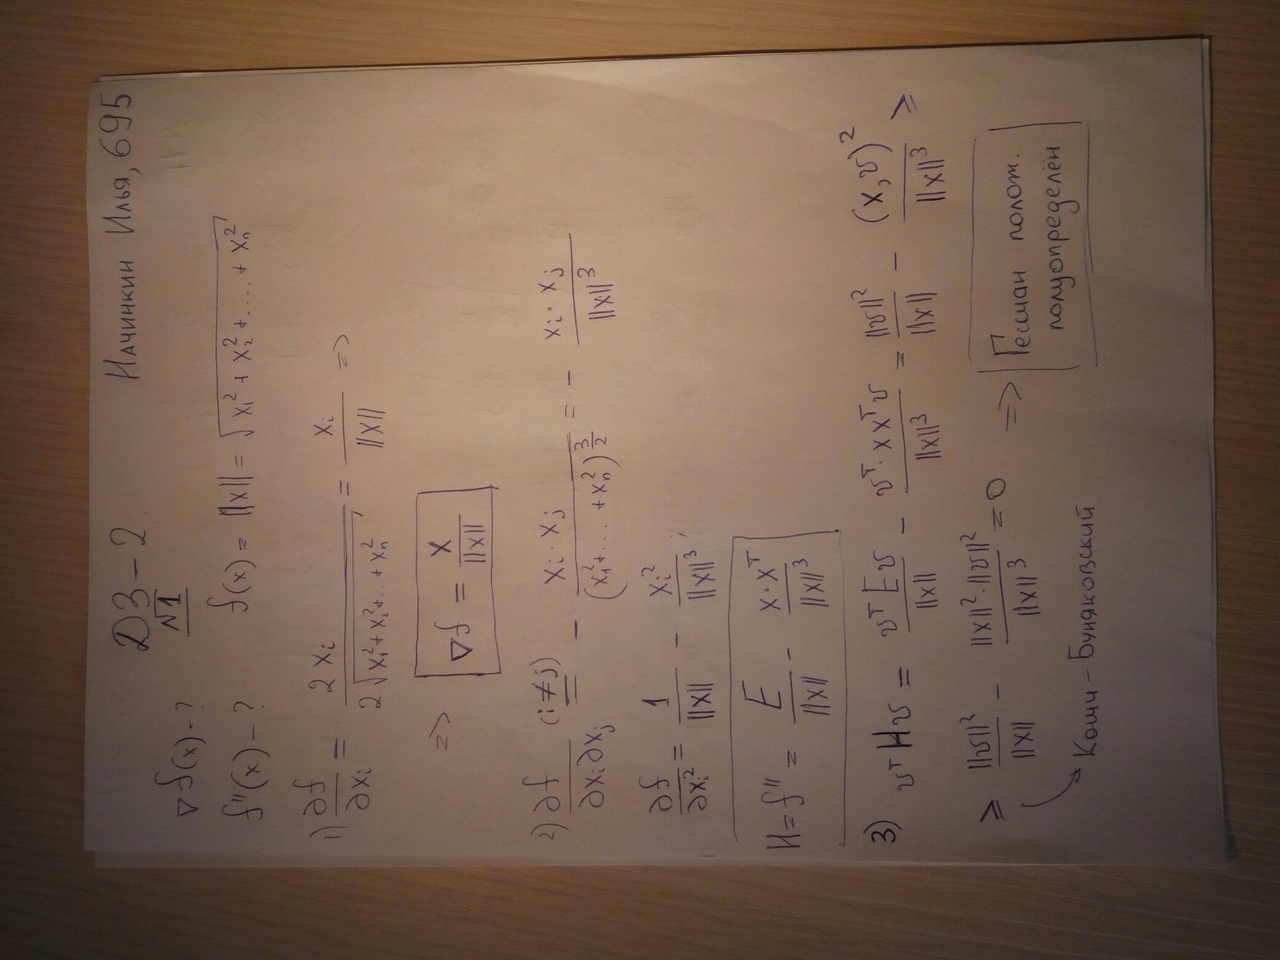
\includegraphics[scale=0.3, angle=270]{one}

\section*{Задача 2}
$f = \norm{(Ax + b)_{+}}$.
\subsection*{Решение}
$$\bigtriangledown{f}(x) = \frac{A^{T}(Ax + b)_{+}}{\norm{(Ax + b)_{+}}} $$
\begin{equation*}
H = f^{''}(x) = \frac{A^{T}Diag(\xi((Ax + b)_{+})A)}{\norm{(Ax + b)_{+}}} - 
\frac{A^{T}(Ax + b)_{+}*(A^{T}(Ax + b)_{+})^{T}}{(\norm{(Ax + b)_{+}})^{3}},
\end{equation*}
 Где $\xi -$ функция от вектора, которые переводит все ненулевые координаты в 1

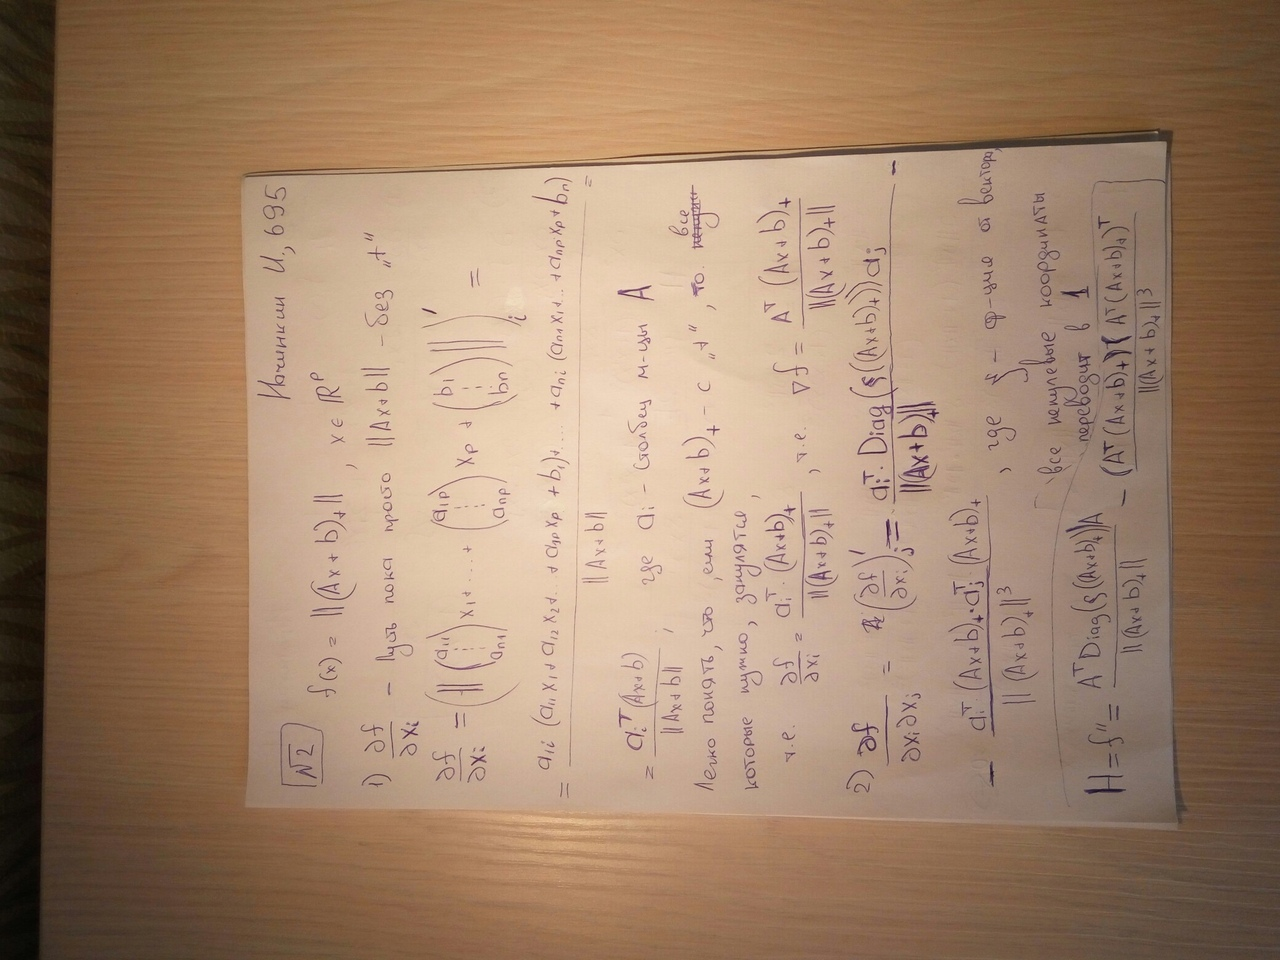
\includegraphics[scale=0.3, angle=270]{two}

\section*{Задача 3}
$f = log(1 + x^{T}Ax), A \geq 0$
\subsection*{Решение}
$$\bigtriangledown{f}(x) = \frac{(A + A^{T})x}{1 + x^{T}Ax}$$

$$H = f^{''}(x) = \frac{(A + A^{T})}{1 + x^{T}Ax} - \frac{(A + A^{T})x*x^{T}((A + A^{T}))}{(1 + x^{T}Ax)^{2}}$$

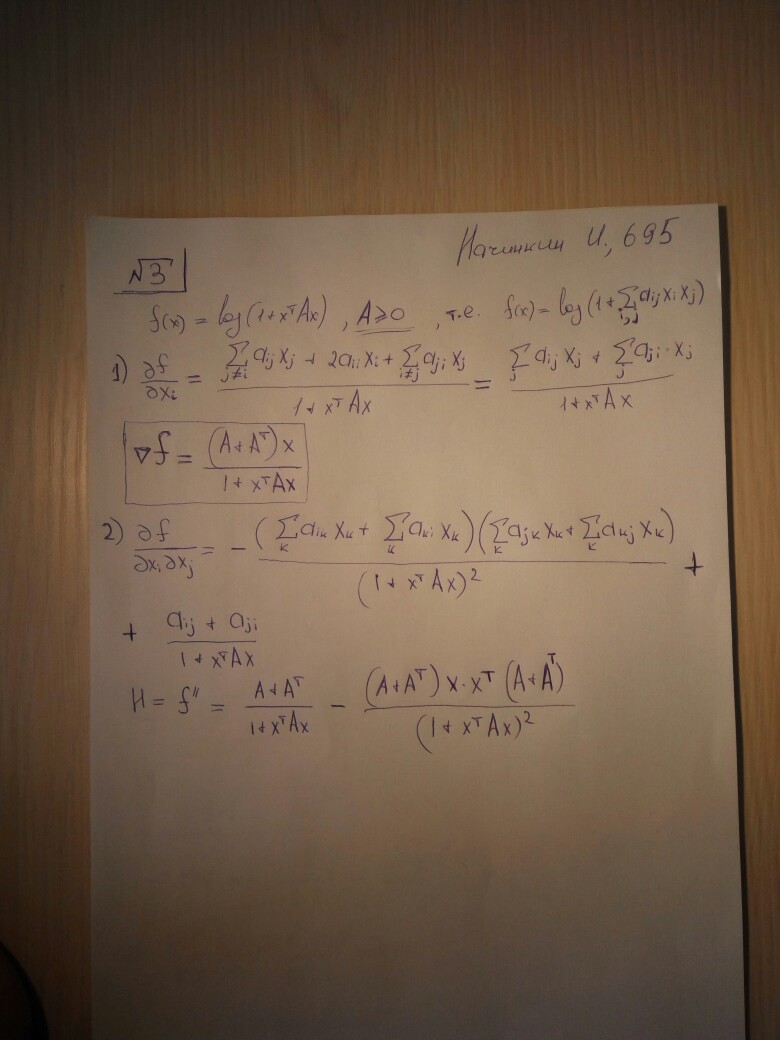
\includegraphics[scale=0.3]{three}

\section*{Задача 4}
$f = \sum_{i=1}^{n}x_{i}log(x_{i}), x \geq 0$
\subsection*{Решение}

\begin{equation*}
\bigtriangledown{f}(x) = 
\begin{pmatrix}
1 \\ 1 \\ ... \\ 1
\end{pmatrix}
+
\begin{pmatrix}
log(x_{1}) \\ log(x_{2}) \\ ... \\ log(x_{n})  
\end{pmatrix}
\end{equation*}

\begin{equation*}
H = f^{''}(x) =  Diag(\frac{1}{x_{1}}, \frac{1}{x_{2}}, ... , \frac{1}{x_{n}})
\end{equation*}

\begin{equation*}
v^{T}Diag(\frac{1}{x_{1}}, \frac{1}{x_{2}}, ... , \frac{1}{x_{n}})v 
= \sum_{i=1}^{n}\frac{v_i^2}{x_i} \geq 0
\end{equation*}
Значит она положительно полуопределена


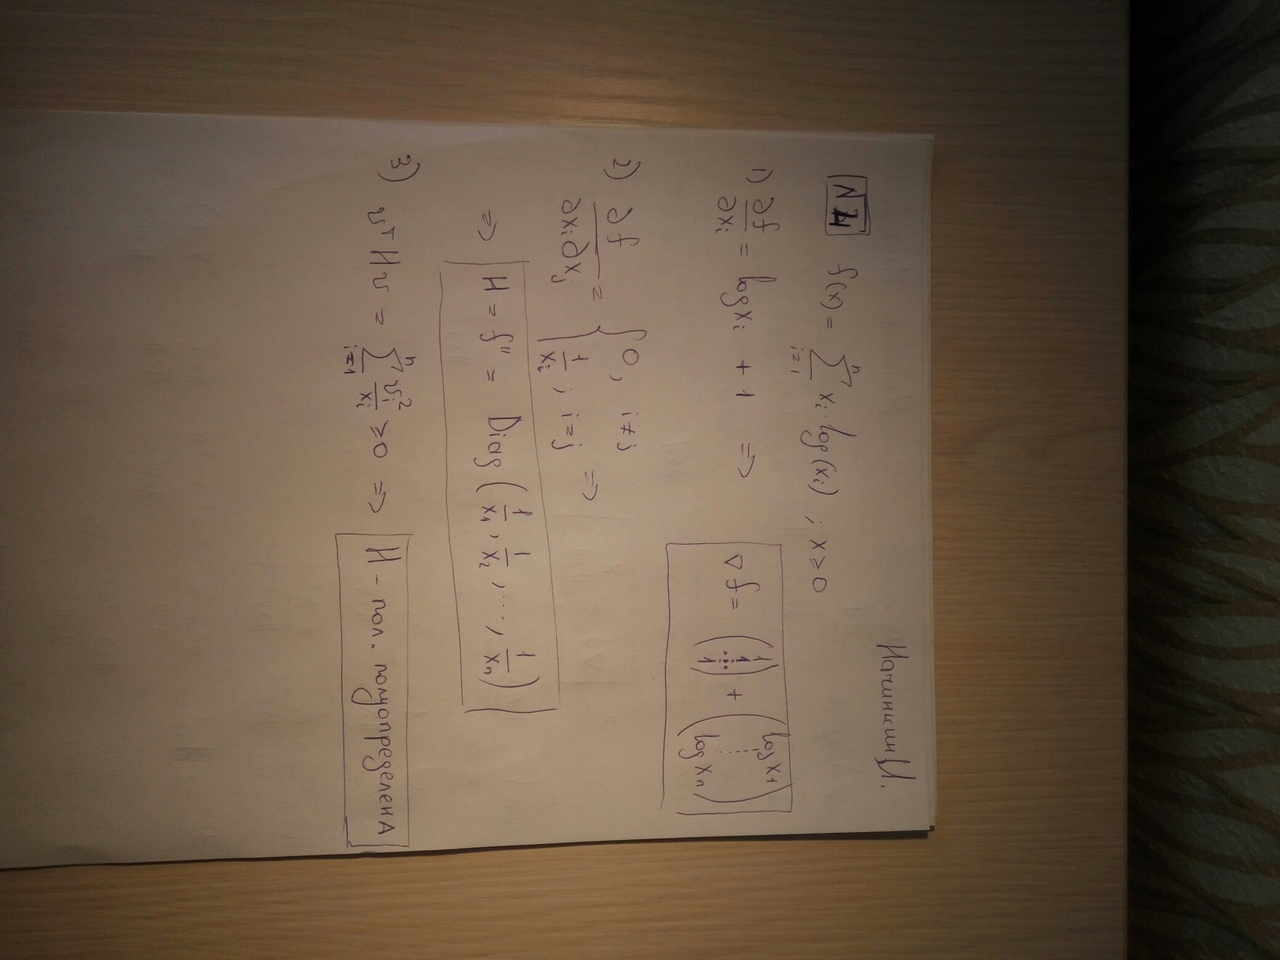
\includegraphics[scale=0.3, angle=90]{four}

\section*{Задача 5}
$f = \frac{-1}{1+x^{T}x}$
\subsection*{Решение}
\begin{equation*}
\bigtriangledown{f}(x) = \frac{2x}{1+x^{T}x}
\end{equation*}

\begin{equation*}
H = f^{''}(x) =  \frac{2E}{(1+x^{T}x)^2} - \frac{8x*x^{T}}{(1+x^{T}x)^3}
\end{equation*}

\begin{equation*}
v^{T}Hv = \frac{2\norm v ^{2}(1 - 3 \norm x ^{2})}{(1 + \norm x ^{2})^{3}} \geq 0
\Longleftrightarrow \norm x ^{2} \leq \frac{1}{3}
\end{equation*}
При таких $x$ гессиан положительно полуопределен.

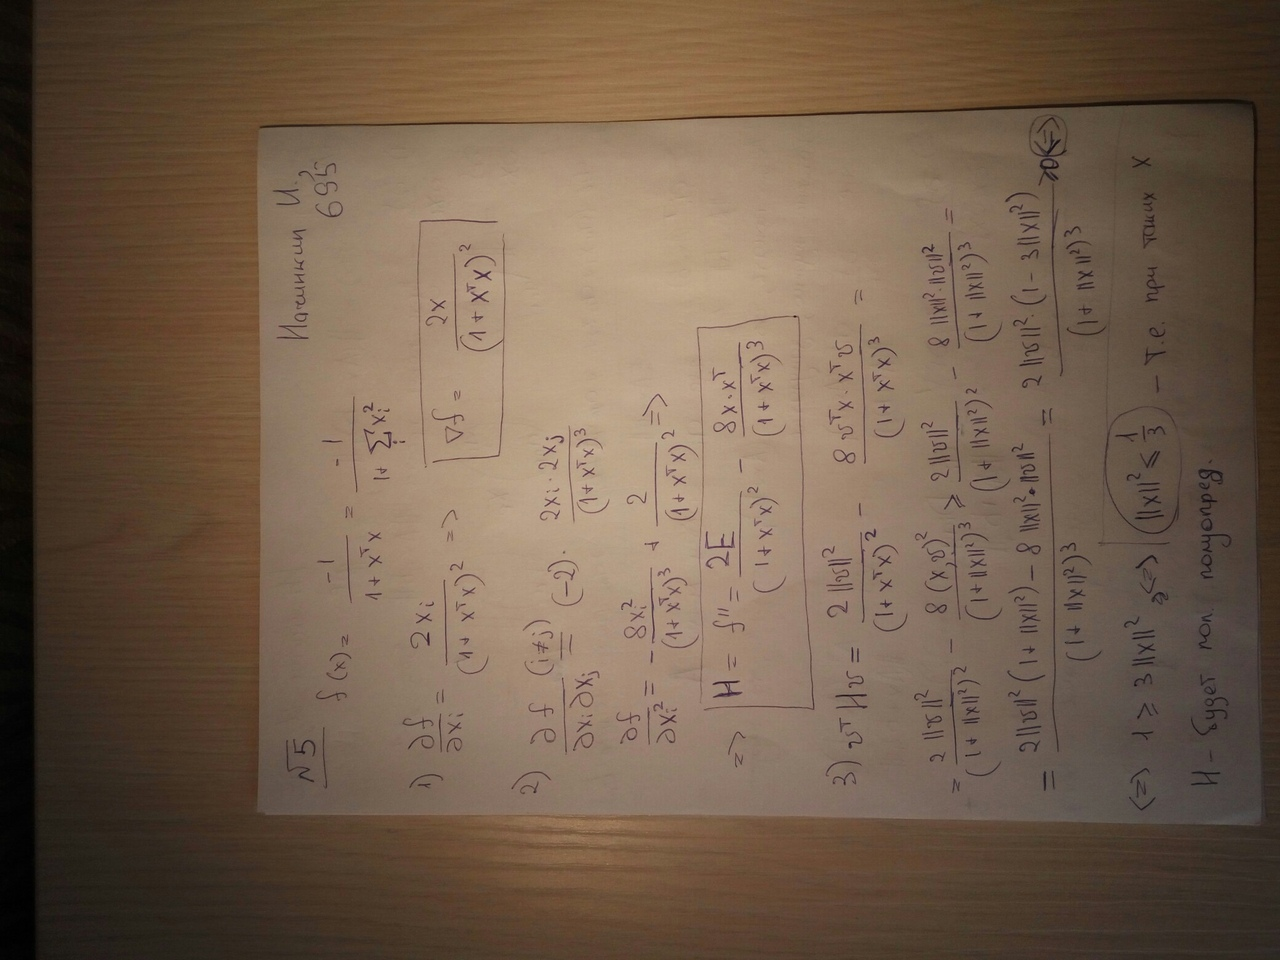
\includegraphics[scale=0.3, angle=270]{five}

\end{document}